\documentclass[aspectratio=169,11pt,t]{beamer}

\usepackage[default]{sourcesanspro}
\usepackage{amsmath,amssymb}
\usepackage{booktabs}
\usepackage{tikz}
\usetikzlibrary{arrows.meta,positioning,calc}

\graphicspath{{../figures/slides/}{../figures/}}

% ----- a plain, light theme -------------------------------------------------
\definecolor{ink}{HTML}{0B0B0B}
\definecolor{ink2}{HTML}{52514E}
\definecolor{rule}{HTML}{E4E3DF}
\definecolor{closed}{HTML}{2A78D6}
\definecolor{open}{HTML}{EB6834}
\definecolor{good}{HTML}{1BAF7A}
\definecolor{soft}{HTML}{F4F3EF}

\setbeamertemplate{navigation symbols}{}
\setbeamercolor{normal text}{fg=ink,bg=white}
\setbeamercolor{structure}{fg=closed}
\setbeamercolor{frametitle}{fg=ink}
\setbeamercolor{title}{fg=ink}
\setbeamercolor{itemize item}{fg=closed}
\setbeamercolor{itemize subitem}{fg=ink2}
\setbeamerfont{frametitle}{size=\Large,series=\bfseries}
\setbeamerfont{itemize/enumerate subbody}{size=\normalsize}
\setbeamertemplate{itemize item}{\raisebox{0.15em}{\rule{0.42em}{0.42em}}}
\setbeamertemplate{itemize subitem}{--}
\setlength{\leftmargini}{1.1em}

\setbeamertemplate{frametitle}{%
  \vspace*{0.9em}%
  \hspace*{-0.1em}\insertframetitle\par
  \vspace*{0.25em}%
  {\color{closed}\rule{2.2em}{2.2pt}}%
  \vspace*{0.1em}%
}
\setbeamertemplate{footline}{%
  \hspace*{1.0em}{\scriptsize\color{ink2}Closing the loop on Jenga}%
  \hfill{\scriptsize\color{ink2}\insertframenumber}\hspace*{1.0em}\vspace*{0.7em}%
}
\setbeamersize{text margin left=1.1em, text margin right=1.1em}

\newcommand{\vect}[1]{\mathbf{#1}}
\newcommand{\muted}[1]{{\color{ink2}#1}}
\newcommand{\bignum}[2]{\begin{minipage}[t]{#1}\centering{\fontsize{30}{32}\selectfont\bfseries #2}\end{minipage}}

\title{Closing the Loop on Jenga}
\subtitle{Visual servoing and force sensing for block extraction, in simulation}
\author{Somanshu Juneja \quad Dharmesh Sahu \quad Pramukto Mandal}
\institute{Indian Institute of Technology Mandi}
\date{}

\begin{document}

% ---------------------------------------------------------------------------
{
\setbeamertemplate{footline}{}
\begin{frame}[c]
\begin{columns}[c]
\begin{column}{0.52\textwidth}
  {\fontsize{26}{30}\selectfont\bfseries Closing the Loop\\on Jenga\par}
  \vspace{0.6em}
  {\large\color{ink2}Visual servoing and force sensing\\for block extraction, in simulation\par}
  \vspace{1.6em}
  {\color{closed}\rule{3em}{2.5pt}}\par\vspace{0.6em}
  Somanshu Juneja \quad Dharmesh Sahu \quad Pramukto Mandal\par
  \vspace{0.2em}
  {\small\color{ink2}Indian Institute of Technology Mandi\par}
\end{column}
\begin{column}{0.46\textwidth}
  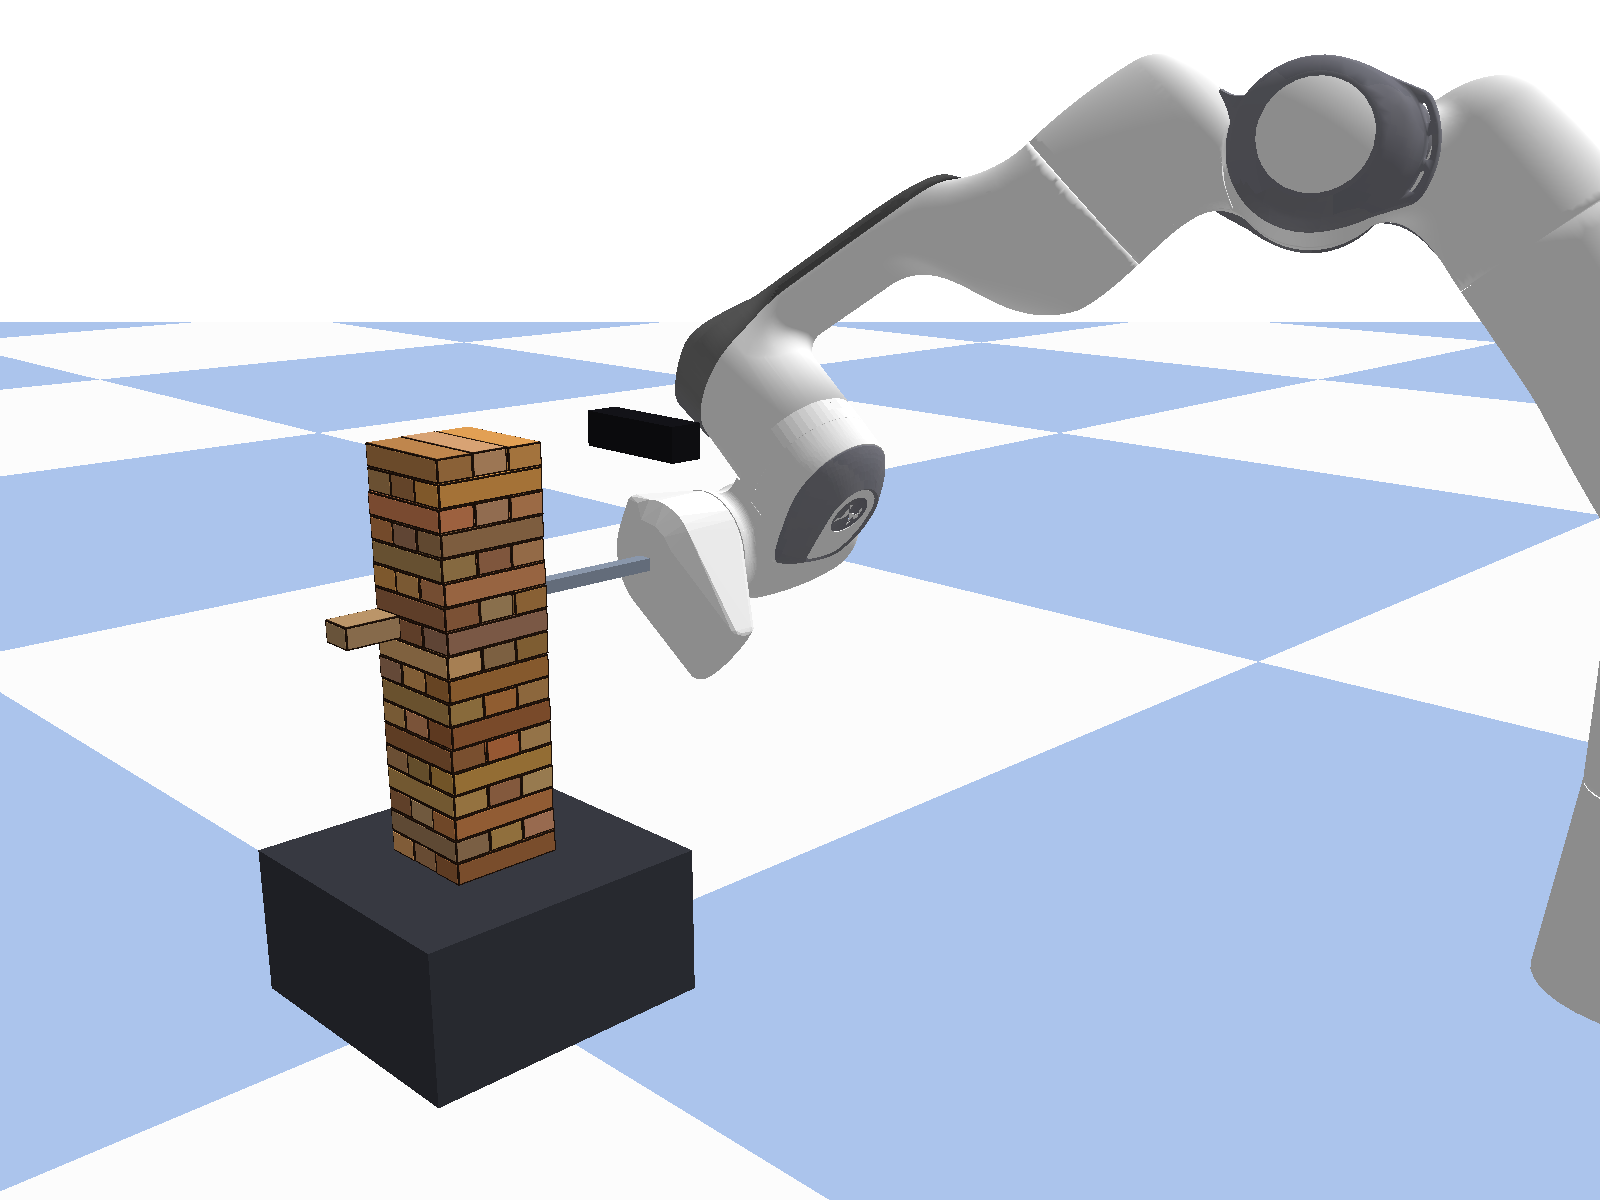
\includegraphics[width=\linewidth]{scene_push_side.png}
\end{column}
\end{columns}
\end{frame}
}

% ---------------------------------------------------------------------------
\begin{frame}{The task}
\begin{columns}[T]
\begin{column}{0.55\textwidth}
Push one block at a time out of an 18-level tower without knocking it over.
\vspace{0.5em}
\begin{itemize}
\item \textbf{Precision.} A 25\,mm face and an 11\,mm fingertip leave about
\textbf{7\,mm} of error before the finger hits a neighbour.
\item \textbf{Vision cannot judge friction.} Whether a block is free depends on
tolerances and the load above it. The robot has to \emph{feel} it.
\item \textbf{The tower gets weaker} with every move.
\end{itemize}
\vspace{0.4em}
\muted{\small Pipeline of Marchionna \emph{et al.} (2023), rebuilt in simulation.}
\end{column}
\begin{column}{0.42\textwidth}
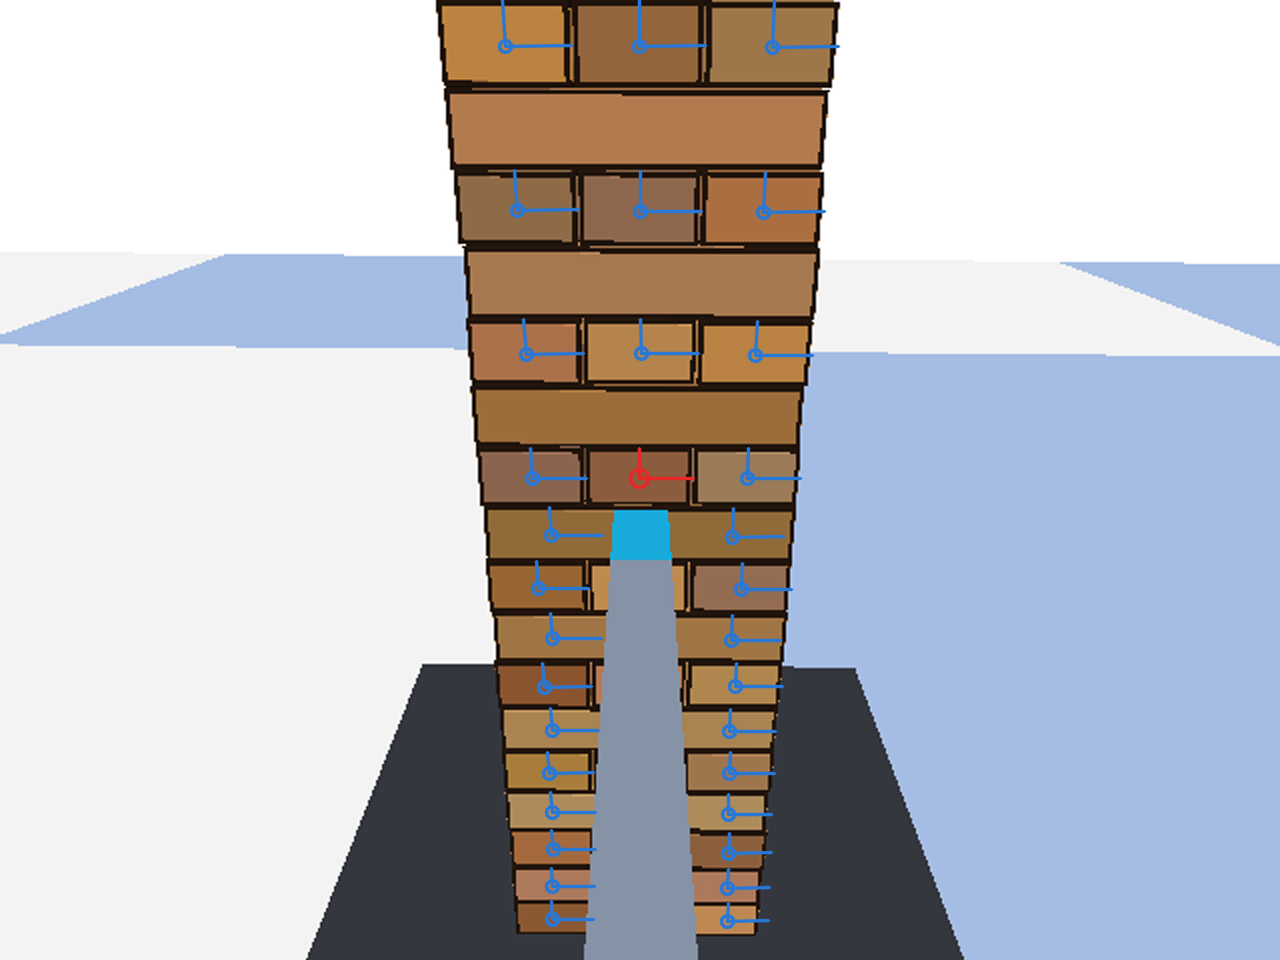
\includegraphics[width=\linewidth]{camera_aligned.png}\par
{\scriptsize\color{ink2}The camera on the arm, after alignment. Target face in red.}
\end{column}
\end{columns}
\end{frame}

% ---------------------------------------------------------------------------
\begin{frame}{Question}
\vspace{2.2em}
\begin{center}
{\Large How much does \textbf{closing the loop with vision} matter,\\[0.3em]
and how good does the \textbf{detector} have to be?}
\end{center}
\vspace{1.8em}
\begin{columns}[T]
\begin{column}{0.45\textwidth}
\centering
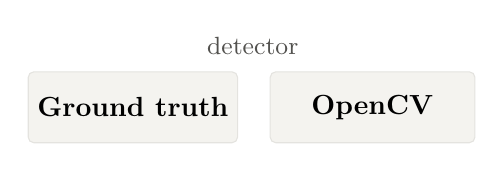
\begin{tikzpicture}
\node[draw=rule, fill=soft, rounded corners=2pt, minimum width=2.6cm, minimum height=0.9cm] (a) {\textbf{Ground truth}};
\node[draw=rule, fill=soft, rounded corners=2pt, minimum width=2.6cm, minimum height=0.9cm, right=0.4cm of a] (b) {\textbf{OpenCV}};
\node[above=0.55cm of $(a)!0.5!(b)$, font=\small, text=ink2] {detector};
\end{tikzpicture}
\end{column}
\begin{column}{0.08\textwidth}\centering\vspace{0.3em}{\Large$\times$}\end{column}
\begin{column}{0.45\textwidth}
\centering
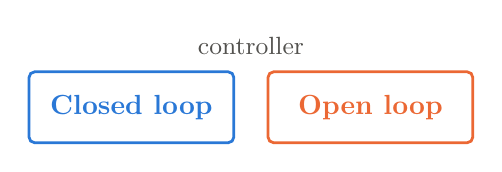
\begin{tikzpicture}
\node[draw=closed, line width=1pt, rounded corners=2pt, minimum width=2.6cm, minimum height=0.9cm] (a) {\textbf{\color{closed}Closed loop}};
\node[draw=open, line width=1pt, rounded corners=2pt, minimum width=2.6cm, minimum height=0.9cm, right=0.4cm of a] (b) {\textbf{\color{open}Open loop}};
\node[above=0.55cm of $(a)!0.5!(b)$, font=\small, text=ink2] {controller};
\end{tikzpicture}
\end{column}
\end{columns}
\vspace{1.4em}
\begin{center}
\muted{4 setups $\times$ 18 games, each game on the same tower in all four setups}
\end{center}
\end{frame}

% ---------------------------------------------------------------------------
\begin{frame}{Simulated system}
\begin{columns}[T]
\begin{column}{0.5\textwidth}
\begin{itemize}
\item \textbf{PyBullet}, 240\,Hz physics, 300 solver iterations
\item \textbf{Franka Panda}, 7-DOF, hand replaced by a 170\,mm finger
\item \textbf{Force sensor}: fingertip on a 100\,N/m spring joint,
read at 20\,Hz, 12-bit
\item \textbf{RGB-D camera} on the arm, 640$\times$480
\item \textbf{Tower}: 54 blocks, $75\times25\times15$\,mm, 19.6\,g, $\mu=0.4$
\end{itemize}
\end{column}
\begin{column}{0.48\textwidth}
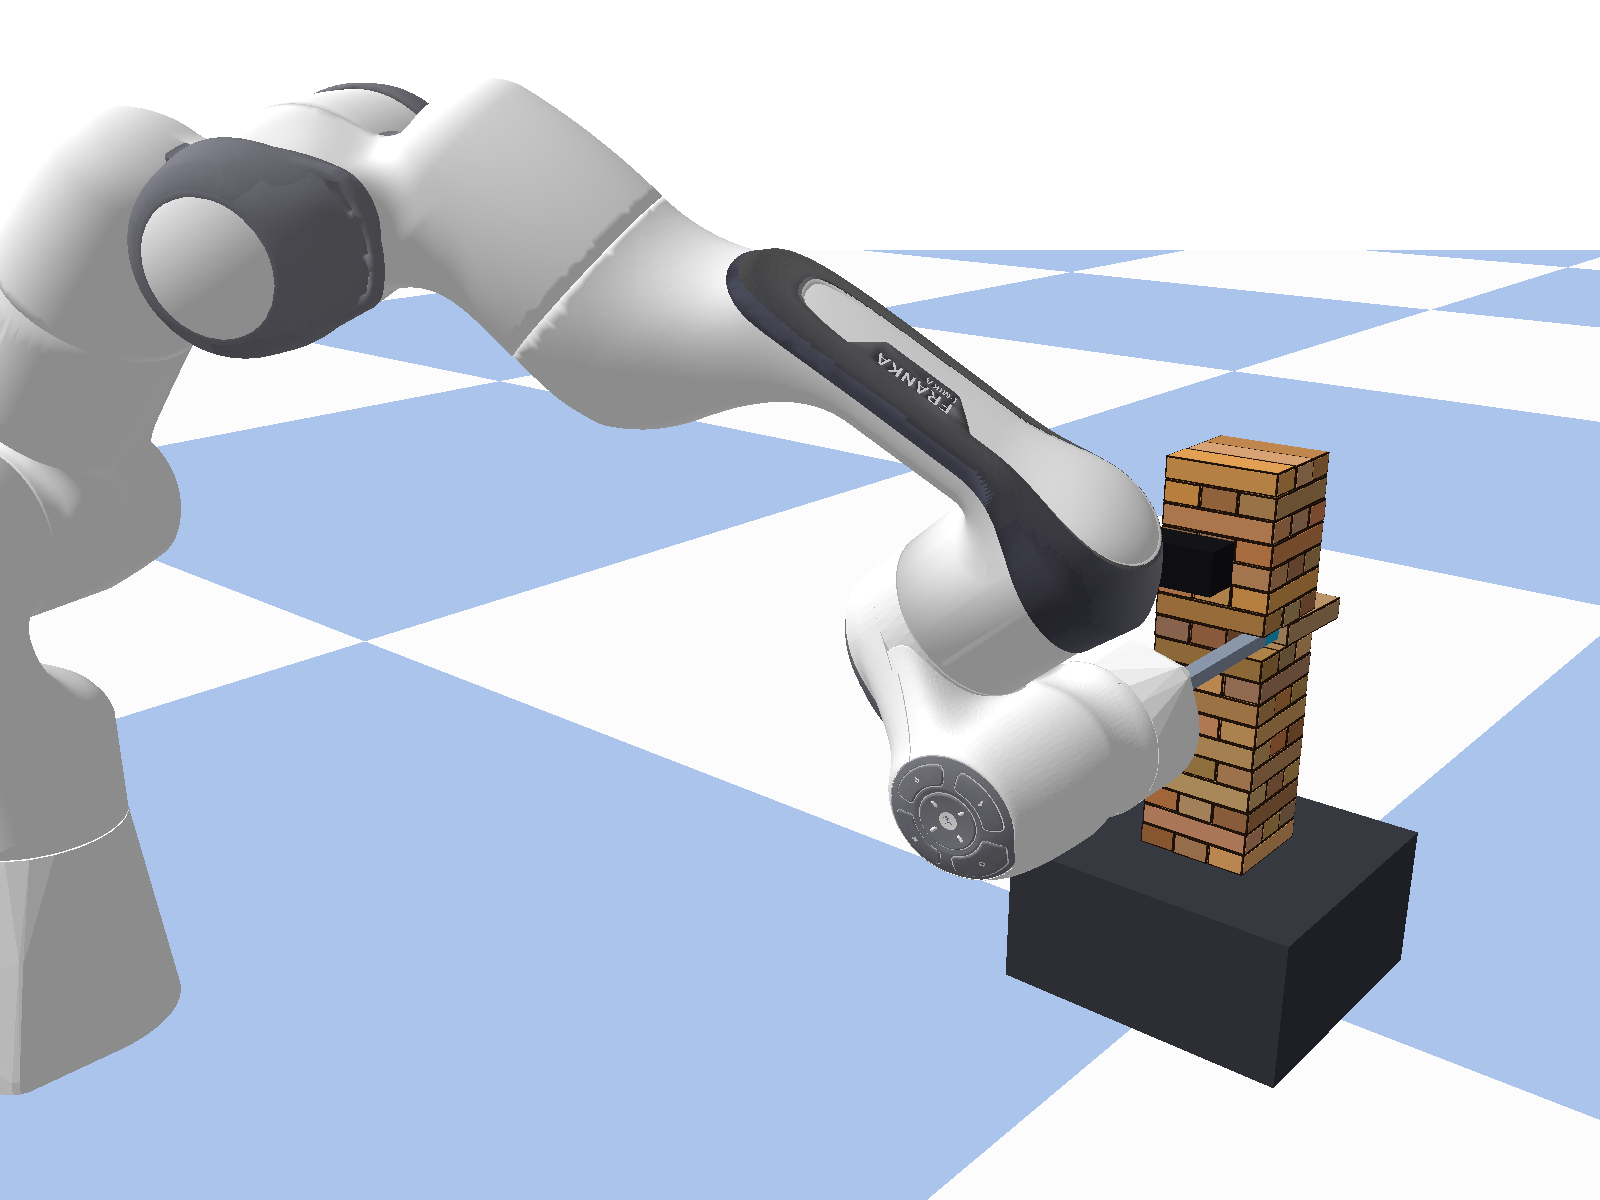
\includegraphics[width=\linewidth]{scene_push_front.png}
\end{column}
\end{columns}
\end{frame}

% ---------------------------------------------------------------------------
\begin{frame}{One attempt, four stages}
\vspace{2.2em}
\centering
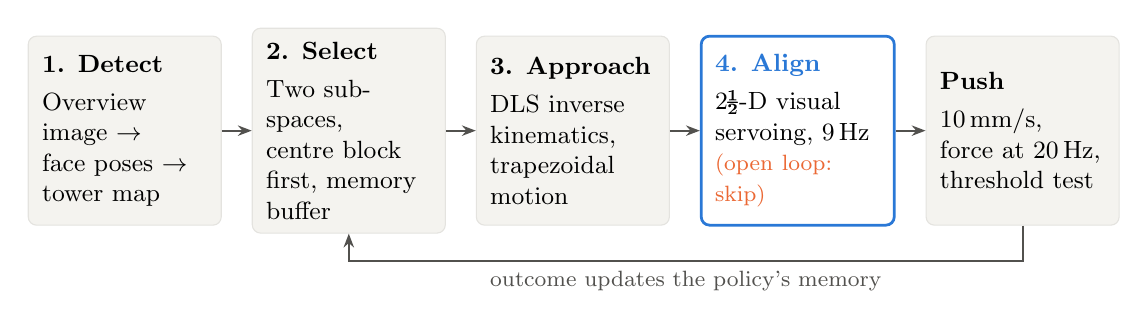
\begin{tikzpicture}[
  st/.style={draw=rule, fill=soft, rounded corners=3pt, text width=2.1cm, minimum height=2.4cm,
             align=left, font=\small, inner sep=5pt},
  arr/.style={-{Stealth[length=5pt]}, draw=ink2, line width=0.8pt}]
\node[st] (a) {\textbf{1. Detect}\\[0.3em] Overview\\ image $\rightarrow$\\ face poses $\rightarrow$\\ tower map};
\node[st, right=0.38cm of a] (b) {\textbf{2. Select}\\[0.3em] Two sub-spaces,\\ centre block\\ first, memory\\ buffer};
\node[st, right=0.38cm of b] (c) {\textbf{3. Approach}\\[0.3em] DLS inverse\\ kinematics,\\ trapezoidal\\ motion};
\node[st, right=0.38cm of c, draw=closed, line width=1pt, fill=white] (d) {\textbf{\color{closed}4. Align}\\[0.3em] 2\textonehalf-D visual\\ servoing, 9\,Hz\\ {\color{open}\footnotesize(open loop: skip)}};
\node[st, right=0.38cm of d] (e) {\textbf{Push}\\[0.3em] 10\,mm/s,\\ force at 20\,Hz,\\ threshold test};
\foreach \x/\y in {a/b,b/c,c/d,d/e} \draw[arr] (\x) -- (\y);
\draw[arr] (e.south) -- ++(0,-0.45) -| node[pos=0.25, below, font=\footnotesize, text=ink2] {outcome updates the policy's memory} (b.south);
\end{tikzpicture}
\end{frame}

% ---------------------------------------------------------------------------
\begin{frame}{Detection without a neural network}
\begin{columns}[T]
\begin{column}{0.5\textwidth}
\textbf{Ground truth}: face poses from the simulator. An upper bound on perception.
\vspace{0.7em}

\textbf{OpenCV}, never reads simulator poses:
\begin{enumerate}
\item HSV threshold for wood colour
\item cut along depth edges, connected components
\item PnP on each face's corners, refine with a plane fit to depth
\end{enumerate}
\vspace{0.4em}
\textbf{Tower map}: snap faces to the layer/slot grid, then match each to a block.
\end{column}
\begin{column}{0.47\textwidth}
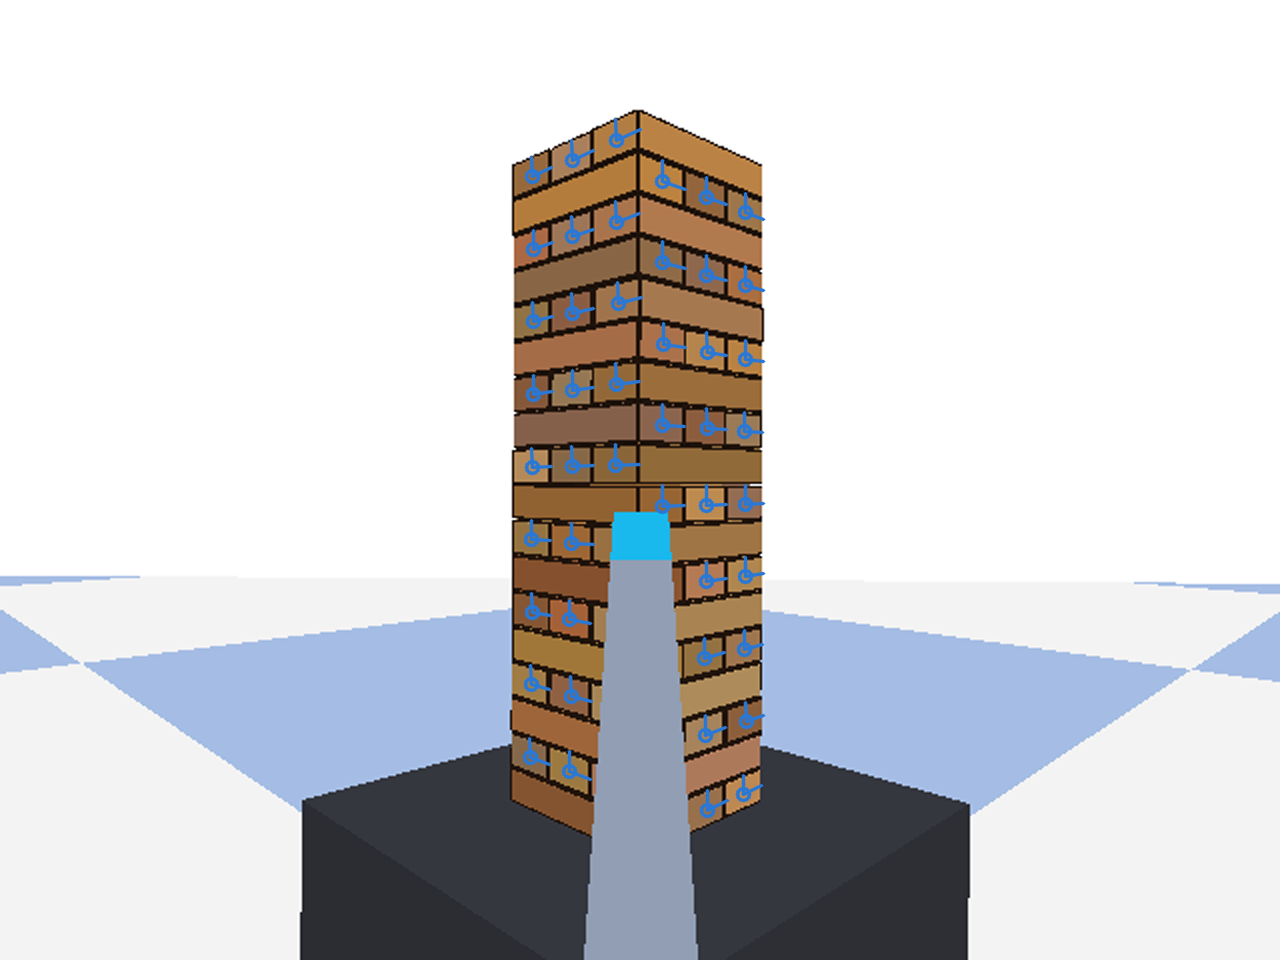
\includegraphics[width=0.9\linewidth]{camera_overview.png}\par
{\scriptsize\color{ink2}Overview image. Circles: detected face centres;\\ lines: estimated face axes.}
\end{column}
\end{columns}
\end{frame}

% ---------------------------------------------------------------------------
\begin{frame}{Aligning the finger: 2\textonehalf-D visual servoing}
\begin{columns}[T]
\begin{column}{0.56\textwidth}
Drive the face's pose in the camera to the pose it has when the fingertip is
25\,mm in front of its centre.
\[
\vect{e} = \big(x-x^{*},\ y-y^{*},\ \log\tfrac{Z}{Z^{*}},\ \theta\vect{u}\big)
\]
\[
\vect{v}_c = -\lambda\,\hat{\vect{L}}^{+}\vect{e}
\qquad
\dot{\vect{q}} = \vect{J}^{+}\vect{v} + (\vect{I}-\vect{J}^{+}\vect{J})\,k(\vect{q}_0-\vect{q})
\]
\begin{itemize}
\item 9\,Hz images, $\lambda=1.5$, stop at 0.5\,mm and 0.005\,rad
\item Redundant 7th joint keeps the arm near its posture
\item \textbf{Open loop} instead moves straight to the target computed from the overview
\end{itemize}
\end{column}
\begin{column}{0.4\textwidth}
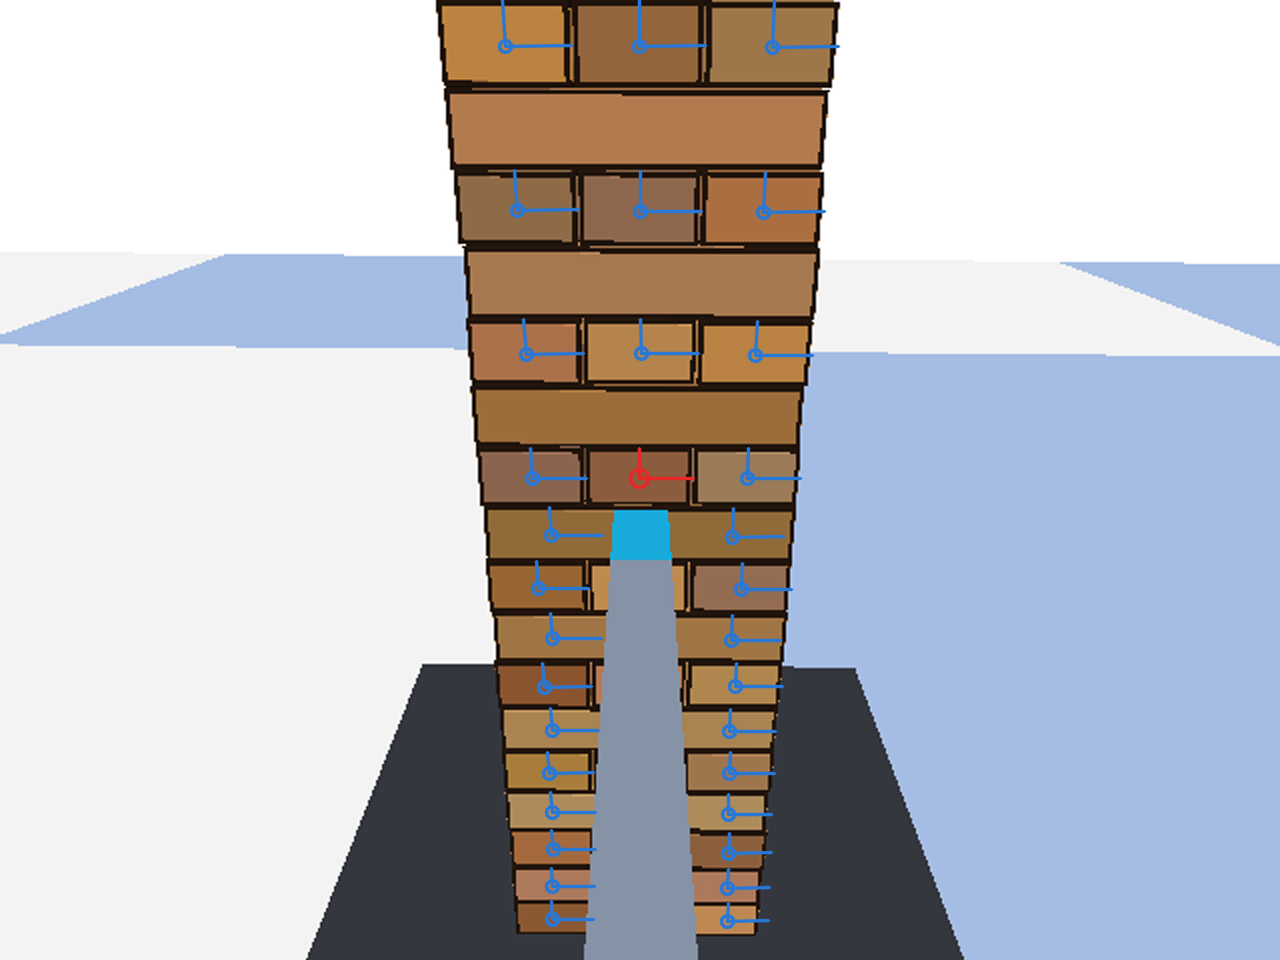
\includegraphics[width=\linewidth]{camera_aligned.png}\par
{\scriptsize\color{ink2}Close-up at convergence. The cyan fingertip sits below the target in the image because the camera looks down from 8\,cm above it.}
\end{column}
\end{columns}
\end{frame}

% ---------------------------------------------------------------------------
\begin{frame}{Feeling the block}
\vspace{-0.3em}
\begin{center}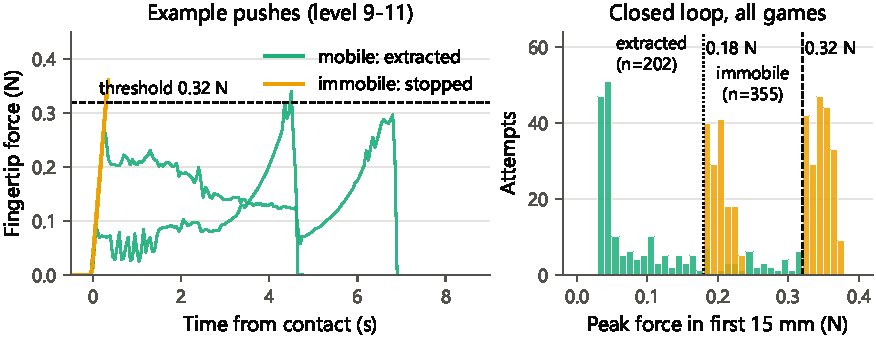
\includegraphics[width=0.84\linewidth]{forces.pdf}\end{center}
\vspace{-0.8em}
\small
\begin{columns}[T]
\begin{column}{0.48\textwidth}
\begin{itemize}
\item Push at 10\,mm/s; \textbf{immobile} if force $\ge$ 0.32\,N (0.18\,N later in the game)
\end{itemize}
\end{column}
\begin{column}{0.48\textwidth}
\begin{itemize}
\item Test only the \textbf{first 15\,mm}. Later, a tipping block drags on the level above,
so a 0.64\,N safety limit applies instead
\end{itemize}
\end{column}
\end{columns}
\end{frame}

% ---------------------------------------------------------------------------
\begin{frame}{Making simulation as hard as reality}
A perfect simulator makes open-loop control look perfect. We add:
\vspace{0.8em}
\begin{columns}[T]
\begin{column}{0.32\textwidth}
\textbf{\color{closed}Block tolerances}\\[0.3em]
\small height $\sigma=0.1$\,mm, position $\pm0.5$\,mm\\[0.3em]
\muted{every tower binds in different places}
\end{column}
\begin{column}{0.32\textwidth}
\textbf{\color{closed}Robot calibration}\\[0.3em]
\small fixed joint-encoder offsets, $\sigma=0.17^\circ$\\[0.3em]
\muted{the robot's model, IK and camera pose are slightly wrong}
\end{column}
\begin{column}{0.32\textwidth}
\textbf{\color{closed}Depth sensor}\\[0.3em]
\small per-pixel noise and a $\pm1\%$ scale error\\[0.3em]
\muted{like a real RGB-D camera}
\end{column}
\end{columns}
\vspace{1.4em}
\begin{block}{}
\small A successful attempt: the block is extracted, or correctly called immobile,
without collapsing the tower. We count them per game.
\end{block}
\end{frame}

% ---------------------------------------------------------------------------
\begin{frame}{Closed loop: about five more successful attempts per game}
\begin{columns}[c]
\begin{column}{0.6\textwidth}
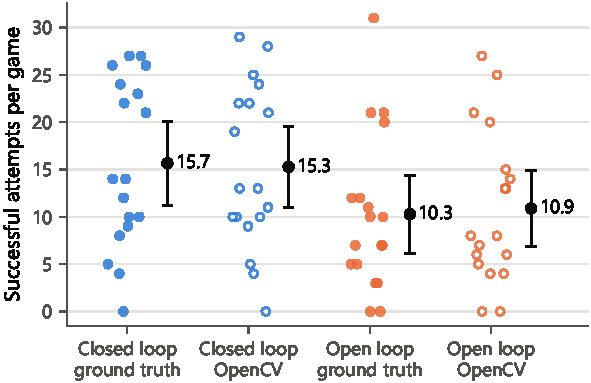
\includegraphics[width=\linewidth]{successes.pdf}
\end{column}
\begin{column}{0.38\textwidth}
\bignum{\linewidth}{\color{closed}15.7\ \ 15.3}\par
\centering\muted{\small closed loop, per game (ground truth, OpenCV)}\par
\vspace{0.8em}
\bignum{\linewidth}{\color{open}10.3\ \ 10.9}\par
\centering\muted{\small open loop}\par
\vspace{0.9em}
\raggedright\small Same tower, both controllers: closed loop wins on 13 of 18 towers with
either detector (sign test $p=0.007$ and $0.02$).
\end{column}
\end{columns}
\end{frame}

% ---------------------------------------------------------------------------
\begin{frame}{Why: alignment}
\vspace{-0.4em}\begin{center}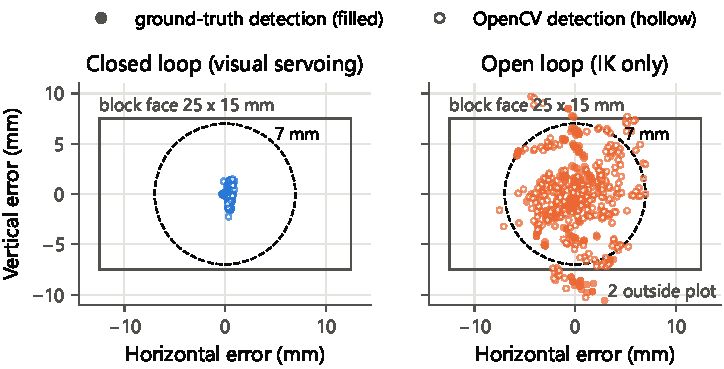
\includegraphics[height=0.6\textheight]{alignment.pdf}\end{center}
\vspace{-0.6em}
\begin{columns}[T]
\begin{column}{0.48\textwidth}
\small\textbf{\color{closed}Closed loop}: 0.14\,mm (ground truth), 0.90\,mm (OpenCV);
every push inside 7\,mm.
\end{column}
\begin{column}{0.48\textwidth}
\small\textbf{\color{open}Open loop}: 3.1 and 4.5\,mm mean, 10--15\,\% outside 7\,mm.
144 errors were pushes on the wrong block.
\end{column}
\end{columns}
\end{frame}

% ---------------------------------------------------------------------------
\begin{frame}{Outcomes}
\begin{columns}[c]
\begin{column}{0.6\textwidth}
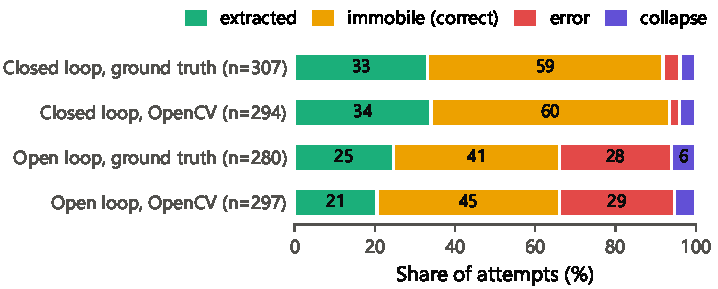
\includegraphics[width=\linewidth]{outcomes.pdf}
\end{column}
\begin{column}{0.37\textwidth}
\small
\begin{itemize}
\item Closed loop: \textbf{92--94\,\%} of attempts succeed
\item Open loop: \textbf{28--29\,\%} are errors, almost all the finger catching a neighbour
\item With the loop closed, OpenCV is as good as perfect detection
(15.3 vs 15.7 per game, $p=0.86$)
\end{itemize}
\end{column}
\end{columns}
\end{frame}

% ---------------------------------------------------------------------------
\begin{frame}{Where blocks come free}
\vspace{-0.4em}\begin{center}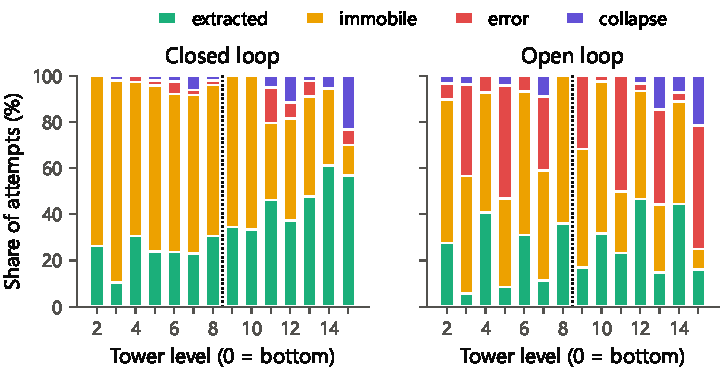
\includegraphics[height=0.54\textheight]{levels.pdf}\end{center}
\vspace{-0.8em}
\small
\begin{itemize}
\item Low levels carry more weight and bind more: 10--31\,\% extracted on levels 2--8,
33--61\,\% on 9--15
\item Collapses cluster at the top; open-loop errors cluster on the odd levels
(faces pointing along $-y$), where calibration error hurts most
\end{itemize}
\end{frame}

% ---------------------------------------------------------------------------
\begin{frame}{Against the physical robot}
\vspace{0.5em}
\centering
\begin{tabular}{@{}lccc@{}}
\toprule
 & \textbf{Physical} & \multicolumn{2}{c}{\textbf{Simulated, closed loop}} \\
 & Marchionna \emph{et al.} & Ground truth & OpenCV \\
\midrule
Successful attempts / game & 13.8 & 15.7 & 15.3 \\
Extractions / game & 7.5 & 5.7 & 5.6 \\
Successful share & 80\,\% & 92\,\% & 94\,\% \\
Most extractions in a game & 14 & 12 & 13 \\
Alignment error & $<$0.2\,mm & 0.14\,mm & 0.90\,mm \\
\bottomrule
\end{tabular}
\vspace{1.2em}
\begin{itemize}
\item Fewer errors in simulation: no lighting, segmentation or workspace-edge failures
\item Fewer extractions: blocks are not stacked back on top, and simulated friction is approximate
\end{itemize}
\end{frame}

% ---------------------------------------------------------------------------
\begin{frame}{What we had to get right}
\begin{itemize}
\item \textbf{Friction needs solver effort.} With fewer than 300 iterations every block looked mobile.
\item \textbf{Score collapses carefully.} A block that tips out of the tower is an extraction,
not a collapse; a block dragged a few mm is a disturbance.
\item \textbf{Calibration error moves everything the camera sees}, differently at each arm
pose. The tower map must be re-registered from every image, and the servo must lock
on by level and slot, not by world position.
\item \textbf{Threshold only while classifying.} Friction rises as a block tips near the end;
a threshold applied to the whole push stops blocks that are almost out.
\end{itemize}
\end{frame}

% ---------------------------------------------------------------------------
\begin{frame}{Limitations and next steps}
\begin{columns}[T]
\begin{column}{0.48\textwidth}
\textbf{Limitations}
\begin{itemize}
\item Simulated, approximate friction
\item Blocks are removed, not restacked
\item Classical detector on rendered images, no trained network
\item One error model; real cameras have structured errors
\end{itemize}
\end{column}
\begin{column}{0.48\textwidth}
\textbf{Next}
\begin{itemize}
\item Learn the block-selection policy (reinforcement learning) using this simulator
\item Larger calibration errors, to map where open loop breaks
\item Restack extracted blocks
\end{itemize}
\end{column}
\end{columns}
\end{frame}

% ---------------------------------------------------------------------------
\begin{frame}{Takeaways}
\vspace{0.8em}
\begin{enumerate}
\setlength{\itemsep}{0.8em}
\item \textbf{Visual servoing is the key component}: under 1\,mm alignment and about
five more successful attempts per game than open loop on the same towers.
\item \textbf{With the loop closed, a classical detector is enough}: it only needs to be
consistent between frames.
\item \textbf{A force threshold over the first 15\,mm} cleanly separates mobile from
immobile blocks.
\end{enumerate}
\vspace{1.6em}
\muted{\small Code, data and figures: \texttt{github.com/tomoeOOseven/jenga-robot-simulation}}
\end{frame}

\end{document}
